\documentclass[12pt,a4paper]{report}
 
\usepackage[brazil]{babel}
\usepackage[utf8]{inputenc}
\usepackage[T1]{fontenc}
\usepackage{graphicx}

\graphicspath{ {images/} }

\title{Solução para captura de análise de sinais analógicos}
\author{Alves, M.\\
	\and
	de Araújo, V.\\
	\and
	Lenza, T.\\
	\and
	Pedreira, M.\\
	\and
	Sandoval, D. A. M.\\
	daniel@loopec.com.br}
\begin{document}
\maketitle
\tableofcontents

\chapter{Introdução}

% Inserir introdução sobre a importância de sinais analógicos e da capacidade de estudá-los

\section{Objetivos}

% Inserir objetivos almejados ao realizar o trabalho

\section{Sinais Analógicos}

%Base de todos os sistemas de telecomunicações;
%Sinais mecânicos: som, sensores;
%Sinais eletromagnéticos: Wi-Fi, Bluetooth, AM, FM, rede elétrica.

\subsection{Transmissão de Dados}

%Dados digitais são modulados em sinais analógicos para transmissão;
%Maior robustez à interferência e atenuação.

\chapter{Projeto de Hardware}

%Aquisição do sinal analógico
%	•	Convertido em sinal elétrico, caso não o seja;
%	•	Amostrado e quantizado;
%Arduino Uno
%	•	Plataforma de desenvolvimento de hardware;
%	•	Baseado no ATmega328;
%	•	2KB SRAM, 1KB EEPROM, 16MHz.
%Aquisição com Arduino
%	•	Detecta variações entre 0-5V;
%	•	1024 níveis;
%	•	800 leituras, a 470Hz.
%	•	Teorema de Nyquist:
%	•	Podemos amostrar sinais de até 235Hz com a taxa de amostragem 470Hz.

\begin{figure}[p]
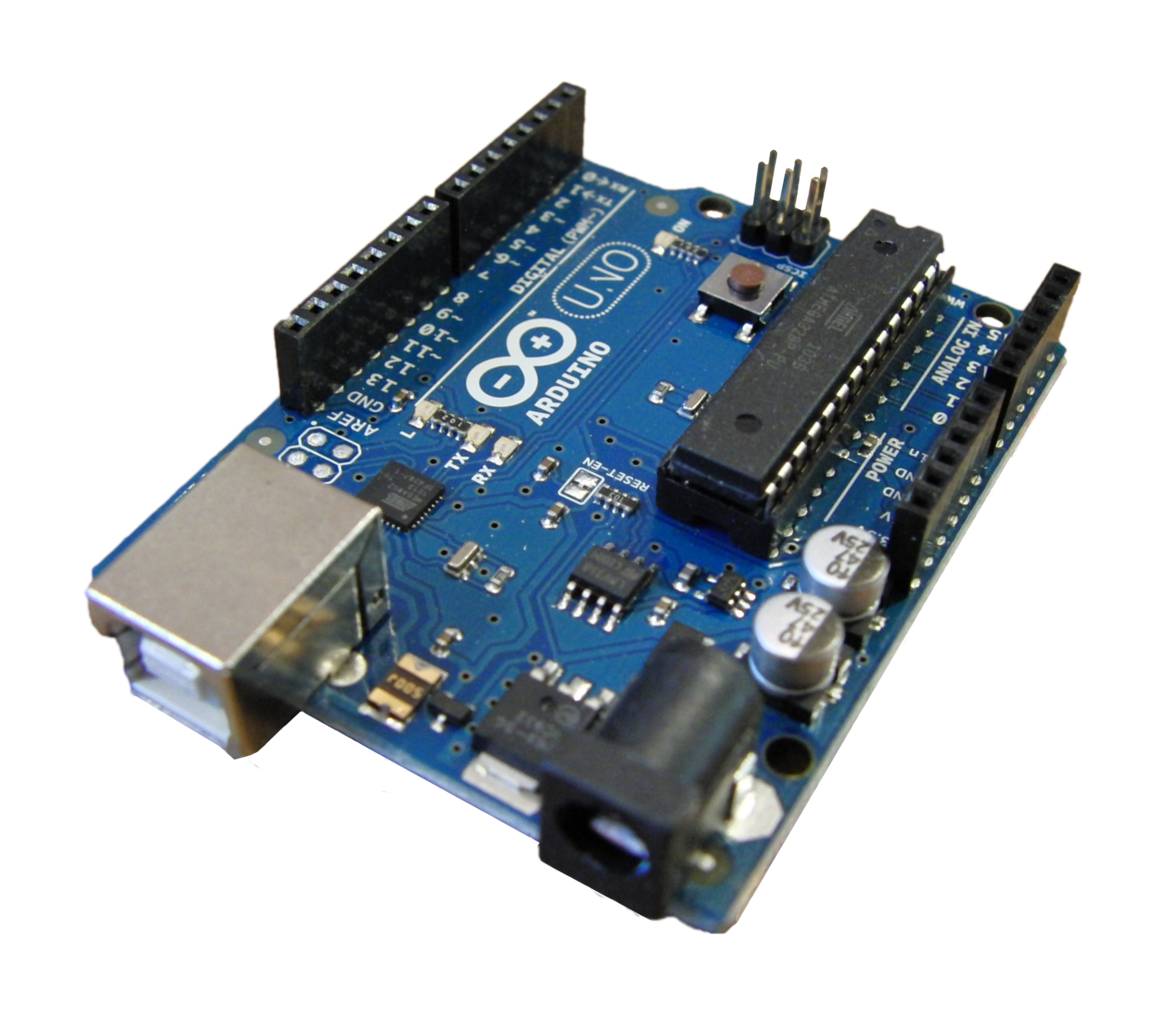
\includegraphics[width=0.8\textwidth]{arduino.png}
\caption{Arduino Uno}
\label{fig:arduino}
\end{figure}

\chapter{Projeto de Software}

%Análise do Sinal
%	•	Recepção dos dados via interface Serial;
%	•	Análise no domínio da frequência;
%	•	Visualização gráfica dos resultados.
%Série de Fourier
%	•	Todo sinal pode ser representado por uma soma de senos e cossenos, denominada Série de Fourier.
%Análise no domínio da frequência
%	•	Sinal é decomposto em sinais periódicos de diferentes amplitudes;
%	•	Transformada rápida de fourier (FFT);
%	•	Observamos a magnitude em cada frequência separadamente.
%INCLUIR INFORMAÇÕES SOBRE PROJETO DO SOFTWARE DE CÁLCULO DA INTEGRAL

\chapter{Resultados}

%Incluir imagens e discutir resultados obtidos.

\end{document}